% Mars Habitat Automation Platform — Presentation Slides
\documentclass[aspectratio=169]{beamer}

\usetheme{Madrid}
\usecolortheme{dove}
\usefonttheme{default}

\usepackage[utf8]{inputenc}
\usepackage[T1]{fontenc}
\usepackage{lmodern}
\usepackage{graphicx}
\usepackage{tikz}
\usetikzlibrary{arrows.meta, positioning, shapes.geometric}
\usepackage{hyperref}
\usetikzlibrary{positioning, arrows.meta, shadows, calc}

\definecolor{marsRed}{RGB}{204,68,68}
\definecolor{marsDark}{RGB}{20,20,30}
\definecolor{marsAccent}{RGB}{255,153,0}

\setbeamercolor{normal text}{fg=black,bg=white}
\setbeamercolor{structure}{fg=marsDark}
\setbeamercolor{title}{fg=white,bg=marsDark}
\setbeamercolor{frametitle}{fg=white,bg=marsDark}
\setbeamercolor{palette primary}{fg=white,bg=marsDark}
\setbeamercolor{palette secondary}{fg=white,bg=marsRed}
\setbeamercolor{palette tertiary}{fg=white,bg=marsDark}
\setbeamercolor{block title}{fg=white,bg=marsDark}
\setbeamercolor{block body}{fg=black,bg=white}
\setbeamercolor{block title example}{fg=white,bg=marsRed}
\setbeamercolor{block body example}{fg=black,bg=orange!8}
\setbeamercolor{footline}{fg=white,bg=marsDark}
\setbeamercolor{page number in head/foot}{fg=white,bg=marsDark}
\setbeamerfont{frametitle}{series=\bfseries,size=\large}
\setbeamerfont{page number in head/foot}{series=\bfseries}
\setbeamerfont{itemize/enumerate body}{size=\small}
\setbeamerfont{itemize/enumerate subbody}{size=\footnotesize}
\setbeamertemplate{blocks}[rounded][shadow=true]
\setbeamersize{text margin left=7mm,text margin right=7mm}
\addtobeamertemplate{itemize/enumerate body begin}{\setlength{\itemsep}{3pt}}{}
\addtobeamertemplate{itemize/enumerate subbody begin}{\setlength{\itemsep}{2pt}}{}

\setbeamertemplate{navigation symbols}{}
\setbeamertemplate{footline}{%
  \leavevmode%
  \hbox{%
    \begin{beamercolorbox}[wd=\paperwidth,ht=2.8ex,dp=1.2ex,leftskip=0.6cm,rightskip=0.6cm]{footline}%
      \hfill\insertframenumber{} / \inserttotalframenumber
    \end{beamercolorbox}%
  }%
}

\title{Mars Habitat Automation Platform}
\subtitle{Distributed Automation for a Simulated Mars Habitat}
\author{MLPG}
\institute{Mars Operations -- Microservices-based IoT Platform}
\date{}

\begin{document}

%======================================================================
\begin{frame}
  \titlepage
\end{frame}

%======================================================================
\begin{frame}{Outline}
  \tableofcontents
\end{frame}

%======================================================================
\section{System Overview}

\begin{frame}{System Description}
  \begin{block}{Goal}
    Provide an automation platform to \textbf{monitor} and \textbf{control} a simulated Mars habitat, starting from sensor data produced by the Mars IoT Simulator.
  \end{block}
  \vspace{0.4cm}
  \begin{itemize}
    \item \textbf{Unified data model}: all raw sensor and actuator signals are normalized into a single \texttt{UnifiedEvent} schema.
    \item \textbf{Event-driven architecture}: services exchange events through a RabbitMQ broker.
    \item \textbf{Automation rules engine}: IF--THEN rules evaluate incoming events and trigger actuator commands.
      \item \textbf{Manual control}: operators can set actuators ON/OFF from the dashboard.
    \item \textbf{Real-time dashboard}: a React SPA (Single Page Application) shows live readings, histories, rule status and conflicts.
  \end{itemize}
\end{frame}

\begin{frame}{High-level Data Flow}
  \centering
  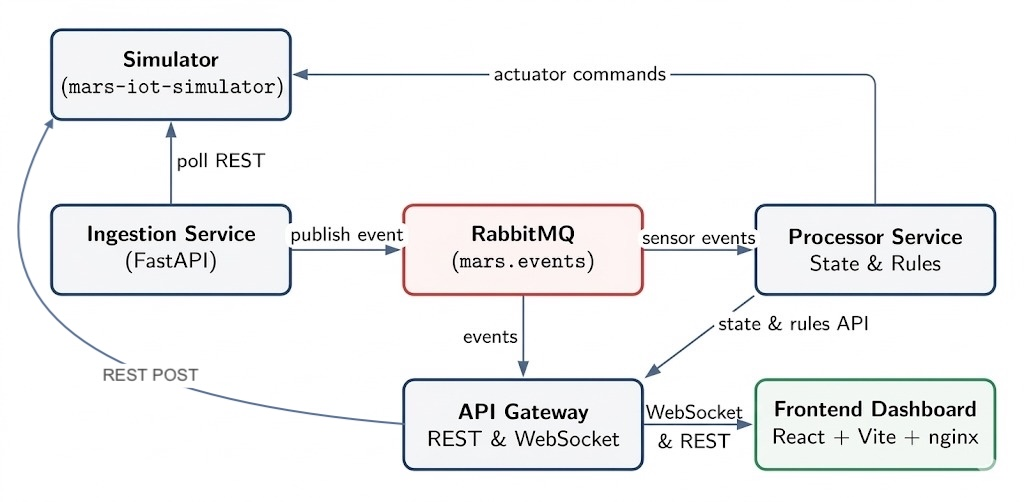
\includegraphics[width=1\textwidth]{architecture_diagram.png}
\end{frame}



%======================================================================
\section{Architecture and Containers}

\begin{frame}{Docker Composition}
  \begin{itemize}
    \item \textbf{simulator} (\texttt{port: 8080}): external Mars IoT Simulator, source of all sensor data and actuators.
    \item \textbf{rabbitmq} (\texttt{ports: 5672}, \texttt{15672}): message broker, exchange \texttt{mars.events}, queues \texttt{processor.events}, \texttt{gateway.events}.
    \item \textbf{ingestion-service} (\texttt{port: 8001}): polls simulator REST (Representational State Transfer, a group of standard rules on how two programs should communicate, e.g. GET, POST, ...) endpoints and publishes normalized events.
    \item \textbf{processor-service} (\texttt{port: 8002}): state cache, rules engine, conflict arbitrator, SQLite persistence, actuator client.
    \item \textbf{api-gateway} (\texttt{port: 8003}): WebSocket endpoint \texttt{/ws}, REST proxies to processor and simulator.
    \item \textbf{frontend} (\texttt{port: 3000}): React SPA served via nginx (Engine-ex); proxies \texttt{/api} and \texttt{/ws} to the gateway.
  \end{itemize}
\end{frame}

\begin{frame}{Ingestion Service Responsibilities}
  \begin{block}{Role in the platform}
    The Ingestion Service is the \textbf{entry point} for all sensor data coming from the Mars IoT Simulator.
  \end{block}
  \vspace{0.15cm}
  \begin{itemize}
    \item \textbf{Polling the simulator}
      \begin{itemize}
        \item Periodically calls the simulator REST endpoints for each sensor (temperature, humidity, particulate, tank levels, \dots).
      \end{itemize}
    \item \textbf{Normalization into \texttt{UnifiedEvent}}
      \begin{itemize}
        \item Converts heterogeneous payloads into the common \texttt{UnifiedEvent} schema.
      \end{itemize}
    \item \textbf{Publishing to RabbitMQ}
      \begin{itemize}
        \item Acts as a producer on the \texttt{mars.events} exchange.
        \item It's fully stateless: in case of restart, it just reconnects and resumes polling the simulator.
      \end{itemize}
  \end{itemize}
\end{frame}

\begin{frame}[t]{Processor Service Responsibilities (1/2)}
  \begin{block}{Core logic engine}
    The Processor Service is the \textbf{brain} of the platform: it tracks latest sensor state and decides when/how to act.
  \end{block}
  \begin{itemize}
    \item \textbf{State management}
      \begin{itemize}
        \item Consumes normalized events from RabbitMQ and updates in-memory \texttt{StateCache}.
        \item Exposes REST endpoints for full/single-sensor state.
      \end{itemize}
    \item \textbf{Rule evaluation}
      \begin{itemize}
        \item Loads automation rules from SQLite and keeps a list of rules.
        \item Evaluates conditions per incoming event and emits logical actuator commands.
      \end{itemize}
  \end{itemize}
\end{frame}

\begin{frame}[t]{Processor Service Responsibilities (2/2)}
  \begin{itemize}
    \item \textbf{Conflict arbitration and safety}
      \begin{itemize}
        \item Uses the \texttt{Arbitrator} to group commands per actuator in a short time window.
        \item Detects ON/OFF conflicts and applies safe-state policy (default: \texttt{OFF}).
      \end{itemize}
    \item \textbf{Persistence}
      \begin{itemize}
        \item Stores rules in SQLite on a Docker volume so configuration survives restarts.
      \end{itemize}
  \end{itemize}
\end{frame}

\begin{frame}[t]{API Gateway and RabbitMQ}
  \begin{block}{API Gateway}
    \begin{itemize}
      \item Provides a \textbf{single entry point} for the frontend.
      \item Exposes \texttt{/ws} for live event streaming.
      \item Proxies \texttt{/api} calls to Processor (state/rules/conflicts) and simulator actuators.
    \end{itemize}
  \end{block}
  \begin{block}{RabbitMQ}
    \begin{itemize}
      \item Central broker for sensor readings, actuator commands, and conflict alerts.
      \item Implements \texttt{mars.events} exchange with service queues.
      \item Decouples ingestion, processing, and streaming so services can scale/restart independently.
    \end{itemize}
  \end{block}
\end{frame}

\begin{frame}[t]{Frontend Dashboard Responsibilities}
  \begin{block}{Operator-facing features}
    \begin{itemize}
      \item Consumes WebSocket events and REST APIs from the gateway.
      \item Renders live sensor cards, actuator states, automation rules, and conflicts.
        \item Supports manual actuator control and rule actions (create/edit/toggle/delete).
    \end{itemize}
  \end{block}
\end{frame}

%======================================================================
\section{Technology Stack}

\begin{frame}[t]{Backend Technology Choices}
  \small
  \begin{block}{Languages and frameworks}
    \begin{itemize}
      \item \textbf{Python 3.11} for all internal services (ingestion, processor, API Gateway).
      \item \textbf{FastAPI} as the main web framework:
        \begin{itemize}
          \item async-first, well aligned with message queues and WebSockets;
        \end{itemize}
    \end{itemize}
  \end{block}
  \vspace{0.1cm}
  \begin{block}{Supporting libraries (AIO versions nd Pydantic)}
    \begin{itemize}
      \item \textbf{aio-pika}: asynchronous RabbitMQ client used by ingestion, processor and gateway to publish/consume events.
      \item \textbf{aiohttp}: async HTTP client to talk to the simulator and to proxy requests between services.
      \item \textbf{aiosqlite}: async SQLite driver used to store/retrieve rules without blocking the event loop.
      \item \textbf{Pydantic}: Ensures that the input data is correct.
    \end{itemize}
  \end{block}
\end{frame}

\begin{frame}{Frontend and UX Technology Choices}
  \begin{block}{Frontend stack}
    \begin{itemize}
      \item \textbf{React 18} for building an interactive single-page dashboard capable of updating without refreshing the page.
      \item \textbf{Vite} as the build tool:
        \begin{itemize}
          \item provides fast development pages
        \end{itemize}
    \end{itemize}
  \end{block}
  \vspace{0.2cm}
  \begin{block}{Serving and integration}
    \begin{itemize}
      \item \textbf{nginx} serves the built static assets and proxies:
        \begin{itemize}
          \item REST requests under \texttt{/api} to the API Gateway;
          \item WebSocket connections under \texttt{/ws} to the same gateway.
        \end{itemize}
      \item The frontend maintains its own in-memory state and histories, reacting to messages from the WebSocket and updates from REST.
    \end{itemize}
  \end{block}
\end{frame}

\begin{frame}{Infrastructure Components}
  \begin{block}{Message broker}
    \begin{itemize}
      \item \textbf{RabbitMQ 3-management} is used as the central event bus.
      \item Defines the \texttt{mars.events} exchange and service-specific queues.
    \end{itemize}
  \end{block}
  \vspace{0.2cm}
  \begin{block}{Database}
    \begin{itemize}
      \item \textbf{SQLite} is chosen for persistence of automation rules:
        \begin{itemize}
          \item embedded and lightweight; no external database service is required.
          \item mounted on a Docker volume to survive container restarts.
        \end{itemize}
      \item Only configuration data (rules) are persisted.
    \end{itemize}
  \end{block}
\end{frame}

%======================================================================
\section{User Stories}

\begin{frame}[t]{Complete List of User Stories (1/2)}
  \vspace{0.3cm}
  \begin{enumerate}
    \setlength{\itemsep}{1em} % Aggiunge respiro tra le righe
    \item \textbf{US01} -- As an operator, I want to read sensors data, so that I can monitor the habitat.
    \item \textbf{US02} -- As an operator, I want to normalize sensors data, so that I can process them.
    \item \textbf{US03} -- As an operator, I want to create automation rules, so that I can automate the habitat.
    \item \textbf{US04} -- As an operator, I want to edit/delete existing automation rules, so that I can modify the behavior of the habitat.
    \item \textbf{US05} -- As an operator, I want to switch on/off automation rules, so that I can modify the behavior of the habitat.
    \item \textbf{US06} -- As an operator, I want to save automation rules, so that they persist after a restart.
  \end{enumerate}
\end{frame}

\begin{frame}[t]{Complete List of User Stories (2/2)}
  \vspace{0.3cm}
  \begin{enumerate}
    \setcounter{enumi}{6} % Fa ripartire i numeri dal 7
    \setlength{\itemsep}{1em}
      \item \textbf{US07} -- As an operator, I want to interact manually with actuators, so that I can directly control the habitat.
    \item \textbf{US08} -- As an operator, I want to see the latest sensor readings, so that I can react immediately to critical changes in the habitat.
    \item \textbf{US09} -- As an operator, I want to check sensors status, so that I can detect malfunctions.
    \item \textbf{US10} -- As an operator, I want to see the evolution of sensors data, so that I can understand the behavior of the habitat.
    \item \textbf{US11} -- As the software, I want to show conflicts between automator rules, so that the operator can solve the issue.
  \end{enumerate}
\end{frame}

\begin{frame}{User Stories (1/2): Monitoring and Data}
  \small
  \begin{itemize}
    \item \textbf{US01 -- US02}: \textbf{Read \& Normalize} raw sensor data to enable continuous habitat monitoring.
    \item \textbf{US08}: \textbf{Live Readings} to react immediately to critical environmental changes.
    \item \textbf{US09}: \textbf{Sensor Status} to quickly detect anomalies and malfunctions.
    \item \textbf{US10}: \textbf{Data Evolution} to understand long-term habitat behavior through historical trends.
  \end{itemize}
  \vspace{0.5cm}
  \begin{block}{How we address them}
    Ingestion normalizes simulator data; the processor keeps the latest state; the dashboard shows live sensor cards, status badges and mini-charts.
  \end{block}
\end{frame}

\begin{frame}{User Stories (2/2): Automation, Control and Conflicts}
  \small
  \begin{itemize}
    \item \textbf{US03 -- US06}: \textbf{Rule Lifecycle Management} (create, edit, toggle, persist) to fully automate the habitat behavior.
    \item \textbf{US11}: \textbf{Rule Priority} to ensure critical automations take precedence.
      \item \textbf{US07}: \textbf{Manual Control} to directly interact with actuators.
    \item \textbf{US11}: \textbf{Conflict Detection} to automatically highlight overlapping rules so the operator can resolve them.
  \end{itemize}
  \vspace{0.5cm}
  \begin{block}{How we address them}
    Rules are stored and evaluated by the processor; the dashboard lets operators manage rules and control actuators; conflicts are strictly arbitrated and highlighted in the UI.
  \end{block}
\end{frame}

%======================================================================
\section{Conflict Management Logic}

\begin{frame}[t]{Conflict Resolution -- Intuition}
  \small
  \begin{block}{Context}
    Multiple automation rules can target the \textbf{same actuator} in the same evaluation cycle.
  \end{block}
  \vspace{0.3cm}
  \begin{itemize}
    \item To ensure safety, the system:
      \begin{itemize}
        \item \textbf{groups} rule outcomes by actuator during a small time window and checks if there some rule that want to set an actuator \texttt{ON} and some rule that want to set an actuator \texttt{OFF};
        \item chooses a \textbf{safe default state} and highlights conflicts in the UI.
      \end{itemize}
    \item This logic is entirely implemented in the processor-service \texttt{Arbitrator} component.
  \end{itemize}
\end{frame}

\begin{frame}[t]{Conflict Handling (Backend)}
  \begin{block}{How conflicts are handled}
    \begin{itemize}
      \item When several rules target the same actuator in a short window, the \textbf{Arbitrator} groups commands.
      \item If all rules agree (all \texttt{ON} or all \texttt{OFF}), the actuator is set accordingly.
      \item If there was a previous warning for that actuator, it is cleared automatically.
      \item If at least one rule asks \texttt{ON} and at least one asks \texttt{OFF}, a \textbf{conflict} is detected.
      \item In conflict, the safe default is applied: actuator set to \texttt{OFF}.
    \end{itemize}
  \end{block}
\end{frame}

%======================================================================
\section{Frontend Mockups}

\begin{frame}[t]{Dashboard Layout (Mockup)}
    \centering
    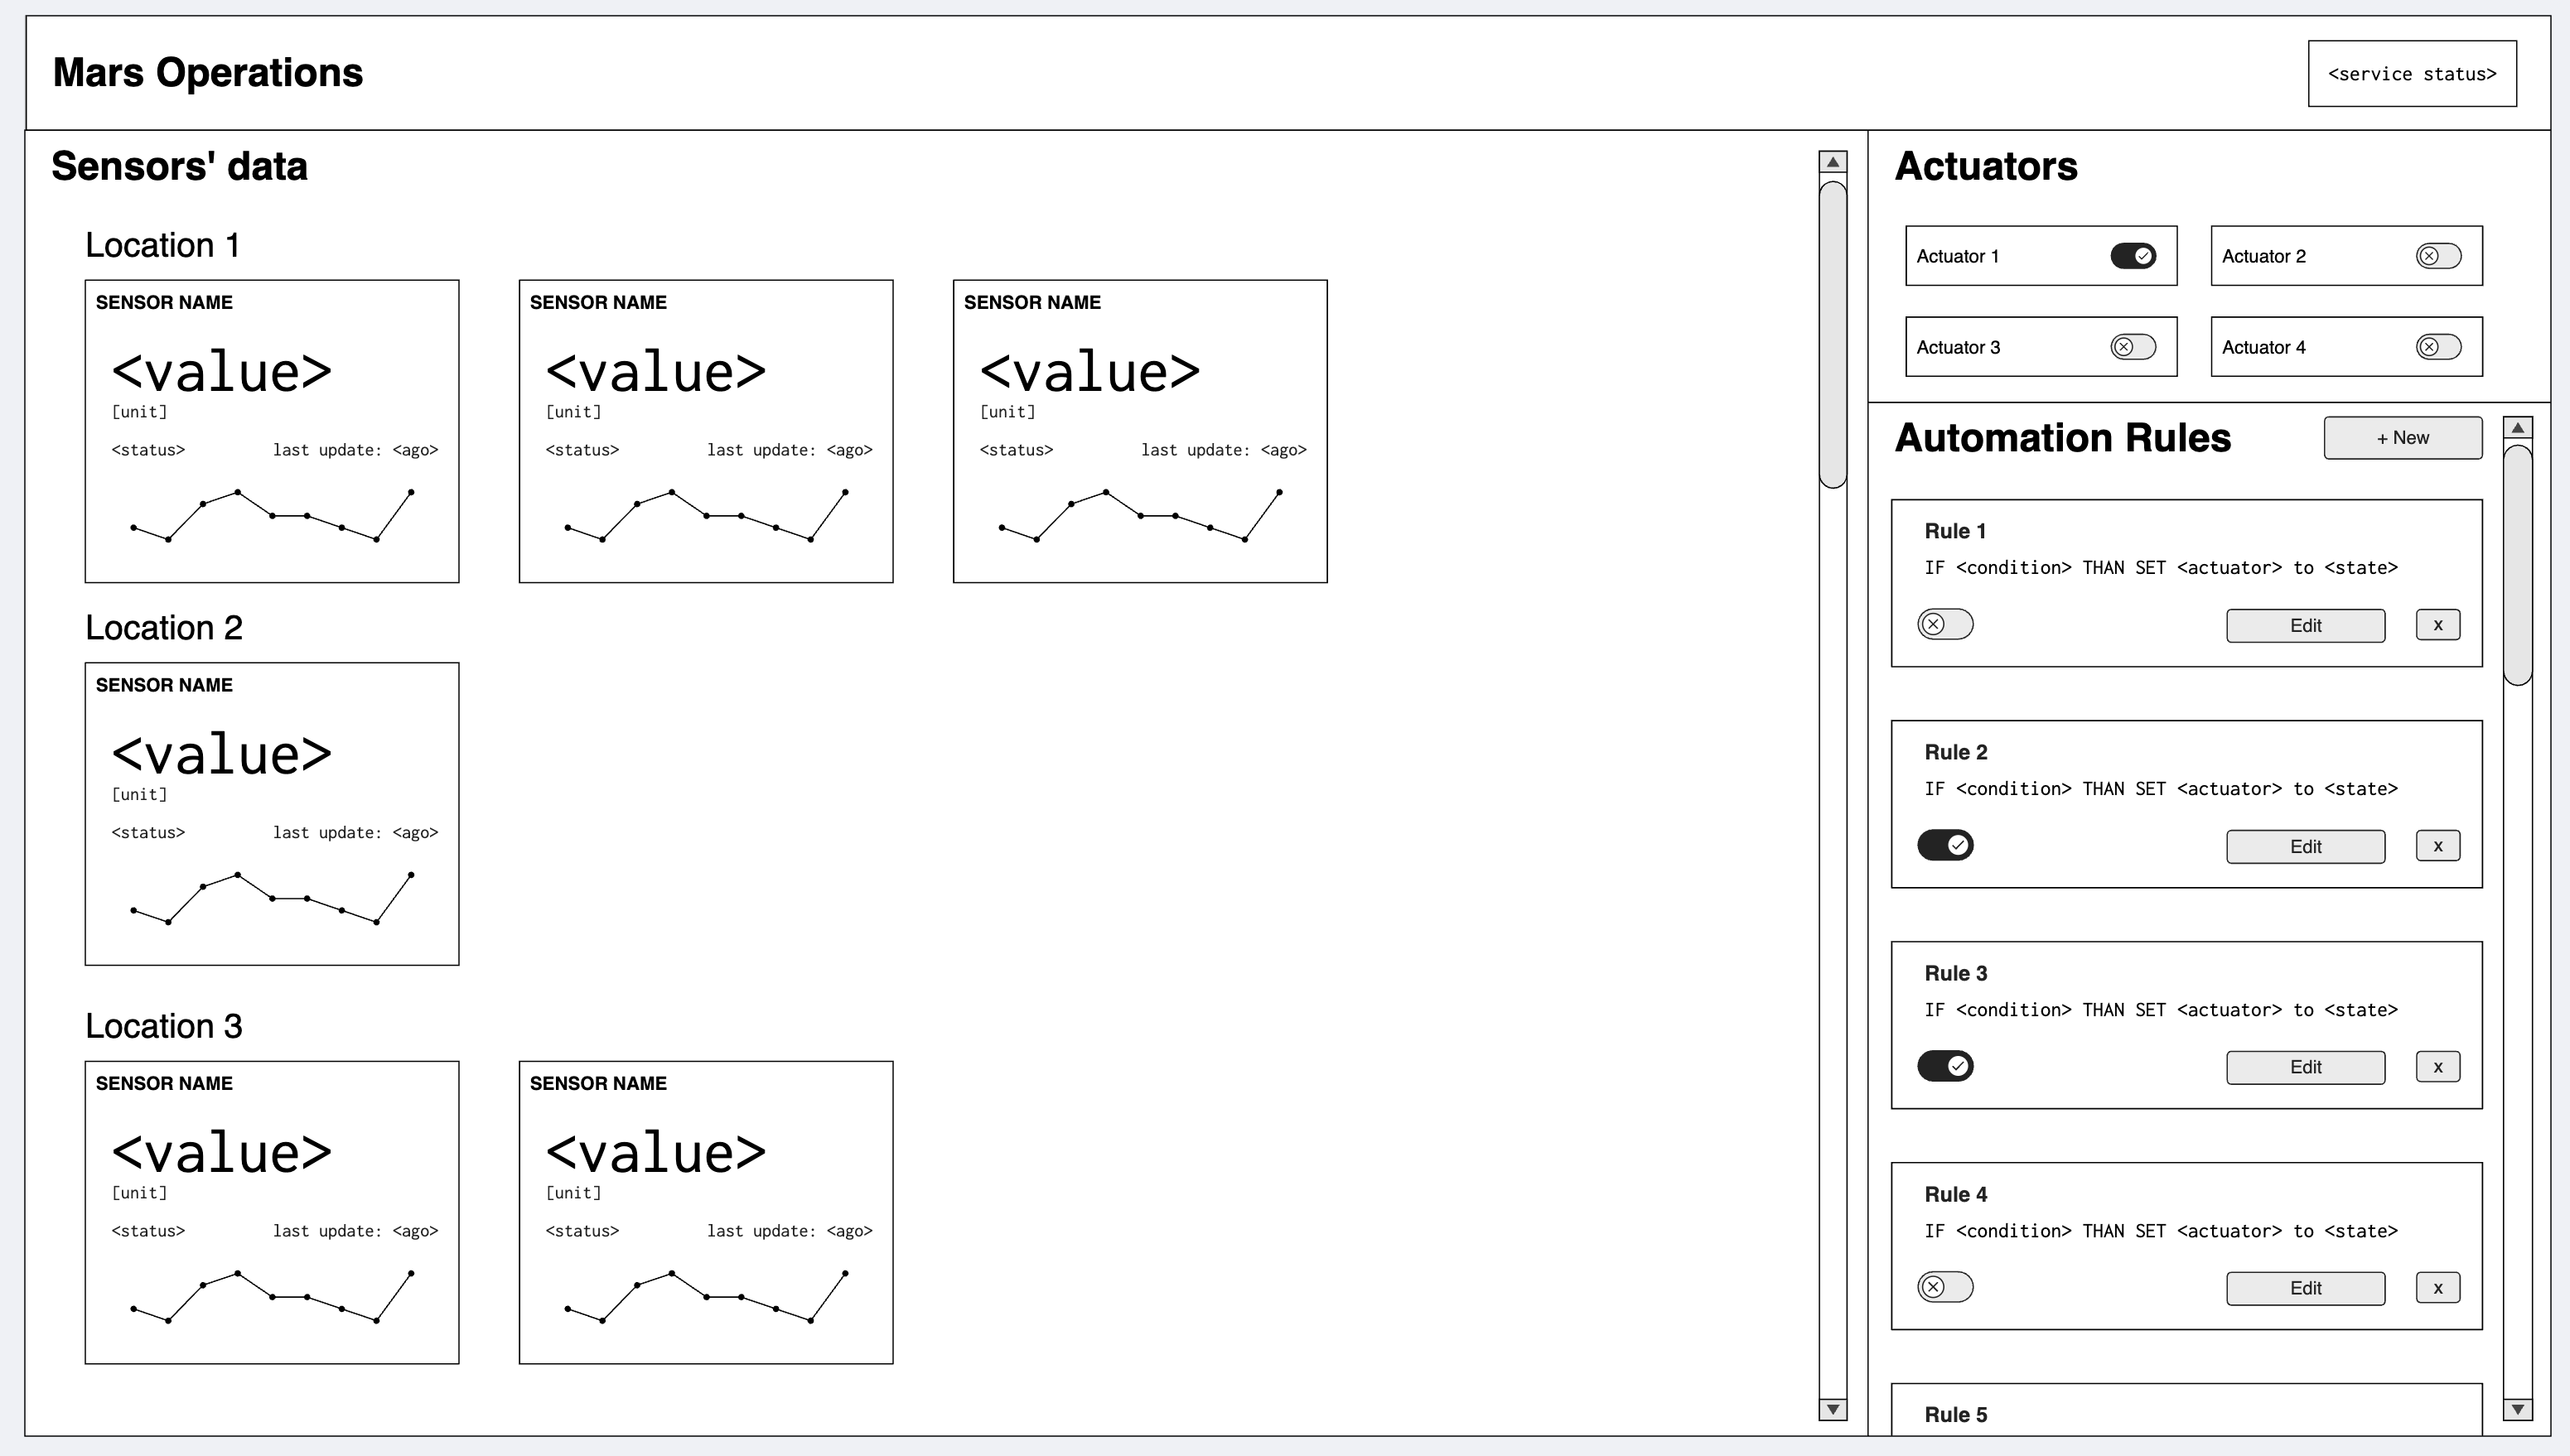
\includegraphics[width=0.8\textwidth]{mockup_home.png}
\end{frame}

\begin{frame}[t]{Sensors Panel (Mockup)}
  \small
  \begin{itemize}
    \item \textbf{Grouping by location}
      \begin{itemize}
        \item Sensors are grouped under headers like \emph{GREENHOUSE}, \emph{ENTRANCE}, \emph{HABITAT}.
        \item Each group can display cards in grid or list view.
      \end{itemize}
    \item \textbf{Sensor cards}
      \begin{itemize}
        \item Show sensor name, location, last value and unit, status indicator and ``last update'' time.
        \item Show a mini SVG chart showing recent history (min/max labels below the chart).
      \end{itemize}
    \item \textbf{Multi-metric sensors}
      \begin{itemize}
        \item For sensors such as \texttt{water\_tank\_level} or \texttt{air\_quality\_pm25}, the card behaves as a small carousel.
        \item Each slide corresponds to a specific metric (e.g. \emph{level pct}, \emph{level liters}, \emph{PM 2.5}).
      \end{itemize}
  \end{itemize}
\end{frame}

\begin{frame}[t]{Actuators Panel (Mockup)}
  \small
  \begin{itemize}
    \item \textbf{Actuator tiles}
      \begin{itemize}
        \item Each actuator (e.g. \emph{cooling fan}, \emph{habitat heater}) appears as a rectangular tile.
        \item Color and icon indicate ON/OFF status at a glance.
      \end{itemize}
    \item \textbf{Interaction}
      \begin{itemize}
          \item Clicking a tile toggles its state and sends a POST request through the API Gateway to the simulator.
          \item WebSocket updates keep tiles synchronized with actual simulator responses.
      \end{itemize}
  \end{itemize}
\end{frame}

\begin{frame}[t]{Automation Rules Panel (Mockup)}
  \small
  \begin{itemize}
    \item \textbf{Rule cards}
      \begin{itemize}
        \item Display the rule name and a readable IF--THEN sentence based on the internal condition.
        \item Include a toggle switch to enable/disable the rule (\texttt{is\_active}).
        \item Provide \emph{Edit} and \emph{Delete} buttons; delete is confirmed with a second click.
      \end{itemize}
    \item \textbf{Create / Edit modal}
    \item \textbf{Conflicts indication}
      \begin{itemize}
        \item Rules involved in active conflicts are highlighted and display a warning icon with a tooltip.
      \end{itemize}
      \begin{itemize}
        \item Guides the user through selecting:
          \begin{itemize}
            \item sensor (and metric, for multi-metric sensors);
            \item comparison operator (\(<, \leq, =, >, \geq\));
            \item threshold value;
            \item target actuator and desired state.
          \end{itemize}
        \item Shows a live textual preview of the resulting rule.
      \end{itemize}
  \end{itemize}
\end{frame}

\begin{frame}[t]{New Automation Rule Layout (Mockup)}
    \centering
    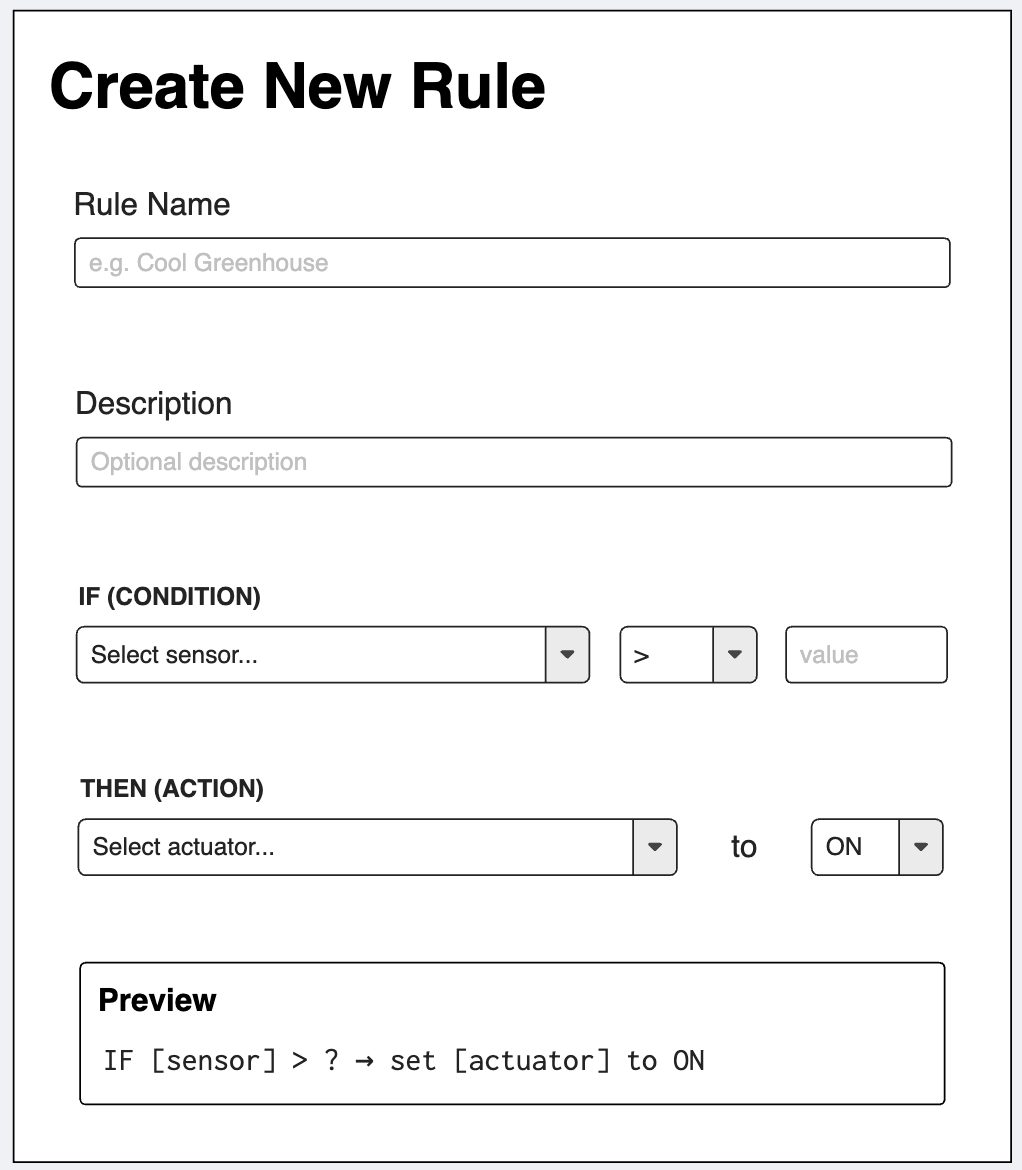
\includegraphics[width=0.4\textwidth]{mockup_new_rule.png}
\end{frame}

%======================================================================
\section{Architecture Summary}

\begin{frame}[t]{Technical Architecture Recap (1/2)}
  \small
  \begin{itemize}
    \item \textbf{Data ingestion}
      \begin{itemize}
        \item Ingestion-Service polls the simulator, normalizes payloads into \texttt{UnifiedEvent}, and publishes them to RabbitMQ.
      \end{itemize}
    \item \textbf{Processing and rules}
      \begin{itemize}
        \item Processor-Service consumes events, updates the state cache, evaluates rules and arbitrates actuator commands.
        \item Rules and their metadata are persisted in SQLite.
      \end{itemize}
    \item \textbf{Exposure to operators}
      \begin{itemize}
        \item API-Gateway exposes WebSocket and REST APIs to the frontend.
        \item Frontend displays live data, histories, rule configuration, conflicts and actuators in a single dashboard.
      \end{itemize}
  \end{itemize}
\end{frame}

\begin{frame}[t]{Technical Architecture Recap (2/2)}
  \centering
  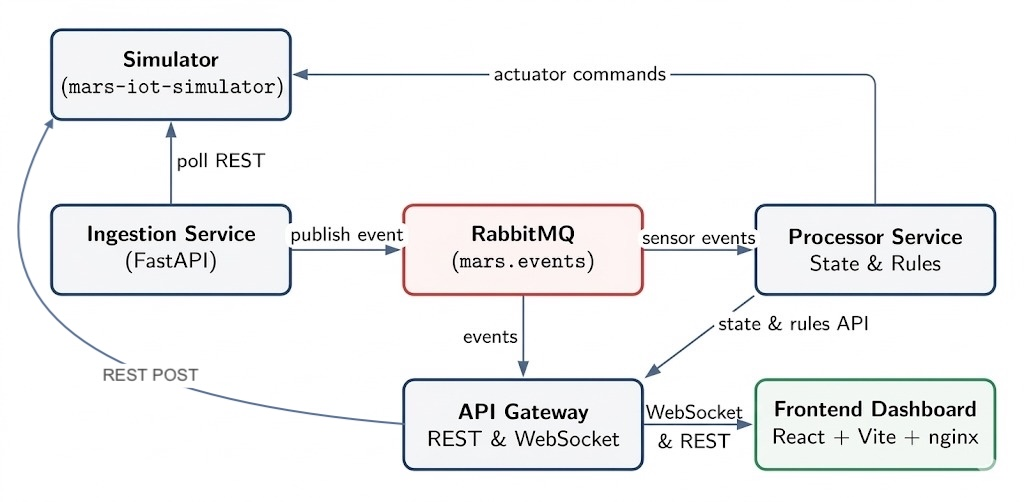
\includegraphics[width=1\textwidth]{architecture_diagram.png}
\end{frame}

\begin{frame}[t]{Example Scenario: Automatic Cooling}
  \small
  \begin{enumerate}
    \item Simulator reports a high \texttt{greenhouse\_temperature} reading.
    \item Ingestion-Service polls the value, builds a \texttt{UnifiedEvent} and publishes it to RabbitMQ.
    \item Processor-Service consumes the event; the rule engine finds a rule such as:
      \begin{quote}
        IF greenhouse temperature \(>\) threshold THEN set cooling fan to ON.
      \end{quote}
    \item The rule triggers and emits a command to the arbitrator; if no conflicting rule asks for OFF, the arbitrator sets the cooling fan to ON.
    \item The actuator command is sent to the simulator and an \texttt{actuator\_command} event is published.
    \item Gateway forwards events via WebSocket; dashboard updates sensors, rule status, and cooling fan tile.
  \end{enumerate}
\end{frame}

%======================================================================

\begin{frame}[c]
  \centering
  \vspace{1cm}
  {\Huge \textbf{Thank You!}} \\
  \vspace{1cm}
  \small \textcolor{marsRed}{MLPG} \\
  \footnotesize Mars Operations -- Microservices-based IoT Platform
\end{frame}

\end{document}